\chapter{Experimentation Methodology}\label{ch:method}

The NFCTP is the first attempt at solving the supply and demand of the nuclear
fuel cycle in a dynamic manner within a NFC simulation. Accordingly, there is no
precedent for investigating the performance and efficacy of a given
approach. This chapter describes one such novel approach in which rules for
generating instances of exchanges are defined, exchanges are generated,
exchanges are executed, and results are analyzed. 

The chapter begins with a discussion of the generation of exchanges, in \S
\ref{method:setup}. Two types of exchanges are included: one in which reactors
are requesting fuel, and one in which reactors are supplying used fuel. In NFC
parlance, these are called the \textit{Front End} of the fuel cycle and
\textit{Back End} of the fuel cycle. Notably, both of these exchanges can occur
in the same time step. \S \ref{method:setup:split} describes how a full exchange
may be split into multiple exchanges for any given time step. 

Generating and solving instances of exchanges at a large scale is a difficult
problem. The Cyclopts (Cyclus Optimization Studies) framework was implemented
for this purpose. Cyclopts has both a Python and C layer. The Python layer is
largely responsible for generating exchanges and interfacing with an associated
persistence mechanism. The C layer is linked against the Cyclus kernel shared
object library and is responsible for calling directly into the kernel's
resource exchange API. \S \ref{method:tools} describes the implementation of
Cyclopts and its varied modes of operation. 

\section{Generating Exchanges}\label{method:setup}

This section focuses on two distinct \textit{species} of exchanges, those
related to the \textit{front end} of the nuclear fuel cycle and those related to
the \textit{back end} of the nuclear fuel cycle. Broadly, the front end of the
fuel cycle is concerned with fueling reactors, and the back end is concerned
with either recycling or disposing of used fuel exiting reactors. Common
features to both types of exchange generation are described in \S
\ref{method:setup:features}.

\S \ref{abm:dre}, however, only describes the methodology for solving a single
exchange. Therefore, an argument must be made for why it is possible to split a
single exchange into multiple exchanges, and specifically why that is valid in
the case of the front and back ends of the NFC. Such an argument is made in \S
\ref{method:setup:split}.

Exchange generation is defined by two types parameters, \textit{exchange} and
\textit{species} parameters. Exchange parameters apply to any species of
exchange, and species parameters apply to a specific species. \S
\ref{method:setup:params} provides a discussion of exchange parameters. \S
\ref{method:setup:front} and \ref{method:setup:back} then follow with a full
description of modeling assumptions and species parameters included for
generating both species of exchanges.

\subsection{Common Features}\label{method:setup:features}

Both species of exchanges include reactors and supporting facilities. In a front
end exchange, supporting facilties are fuel suppliers. In a back end exchange,
supporting facilities are fuel recycling or storage facilities. 

\subsubsection{Fuel Cycles and Commodities}

Three types of fuel cycles can be generated: a once-through fuel cycle (OT), a
plutonium-recycle fuel cycle (MOX), and a plutonium and thorium-recycle fuel
cycle (MOX-ThOX). As fuel cycles increase in complexity, the number of
commodities that exist increases, as shown in Table \ref{tbl:fc_to_commods}. The
commodities are referred to by abbreviation: Enriched Uranium Oxide (UOX), Mixed
Plutonium Oxide for Thermal Reactors (TMOX), Mixed Plutonium Oxide for Fast
Reactors (FMOX), Thorium Oxide for Fast Reactors (FThOX).

\begin{table}[h]
\centering
\caption{A mapping between fuel cycles to their associated commodities.}
\label{tbl:fc_to_commods}
\begin{tabular}{|c|c|}
\hline
Fuel Cycle            & Commodities \\ \hline
OT                    & UOX         \\ \hline
\multirow{3}{*}{MOX}  & UOX         \\  
                      & TMOX        \\  
                      & FMOX        \\ \hline
\multirow{4}{*}{ThOX} & UOX         \\  
                      & TMOX        \\  
                      & FMOX        \\  
                      & FThOX       \\ \hline
\end{tabular}
\end{table}

\subsubsection{Reactors}

All reactors are modeled as either thermal or fast reactors. Thermal reactors
are simplified models of AP-1000 reactors \cite{ARIS}, and fast reactors are
simplified models of BN-600 reactors \cite{reactors2007experience}. Using the
dimensions in Table \ref{tbl:rxtr_params}, one can estimate that the AP-1000 core
volume is approximately 12.5 times larger than the BN-600 core. 

\begin{table}[h]
\centering
\caption{Primary Reactor Parameters}
\label{tbl:rxtr_params}
\begin{tabular}{|c|c|c|c|}
\hline
Reactor & Core Height (m) & Core Diameter (m) & Number of Assemblies \\ \hline
AP1000  & 4.27            & 3.04              & 157 \\ \hline
BN600   & 0.75            & 2.05              & 369 \\ \hline
\end{tabular}
\end{table}

Reactors are assumed to to operate in a batch mode, where each batch is
approximately one quarter of the reactor core, similar to other analyses
\cite{rineiski2011reactivity}. Additionaly, a single AP-1000 fuel assembly is
assumed to contain 450 kg of material \cite{kok2009nuclear}. Therefore, a single
batch of thermal reactor fuel is assumed to be

\begin{equation}
   450 \frac{kg}{assembly} * \frac{t}{1000 \: kg} * 157 \frac{assemblies}{core}
   * \frac{1}{4} core = \: \sim 17.6 t.
\end{equation}

The amount of fuel required and number of assemblies by each reactor type is
shown in Table \ref{tbl:rxtr_batch}. The number of assemblies is taken as the
ratio of total number of assemblies and number of batches per core rounded to
the nearest integer. The batch size for the BN600 reactor is estimated by
dividing the AP1000 batch size by the relative core volume.

\begin{table}[h]
\centering
\caption{Reactor Batch Size}
\label{tbl:rxtr_batch}
\begin{tabular}{|c|c|c|c|}
\hline
Reactor & Quantity (t) & Number of Assemblies \\ \hline
AP1000  & 17.6          & 39 \\ \hline
BN600   & 1.41          & 92 \\ \hline
\end{tabular}
\end{table}
 
\subsubsection{Preferences}

Preferences for all transactions have a default value, $p_{c}(i, j)$, based on
the proposed commodity to be transferred which are defined in species-specific
sections, \S \ref{method:setup:front} and \ref{method:setup:back}. However, a
large exchange with a small preference distribution can lead to problem
degeneracy. Further, a primary application for Cyclus is the modeling of
regional and location effects on fuel cycles. Accordingly, a location proxy is
provided for preferences, as shown in Equation \ref{eqn:loc_proxy}.

Each facility is assigned a location value, $loc_i \in [0, 1)$. The domain is
  then divided evenly into ten regions, where the first region comprises all
  location values in $[0, 0.1)$, and so on. $\delta_{reg}$ and $\delta_{loc}$
    are binary variables which are activated based on the parameters described
    in \S \ref{method:setup:params}. The exponential of the negative absolute
    difference between two regions or locations was chosen as the preference
    function in order to model having higher preferences for closer entities.

\begin{equation}\label{eqn:loc_proxy}
p_{l}(i, j) = \delta_{reg} \frac{\exp(- | reg_{i} - reg_{j} | ) + \delta_{loc}
  \exp(- \| loc_{i} - loc_{j} \| )}{1 + \delta_{loc}}
\end{equation}

The preference for a given arc is then a weighted combination of location and
commodity preferences as shown in Equation \ref{eqn:total_pref}. The weighting
factor, $r_{l, c}$, is a parameter of exchange generation and described further
in \S \ref{method:setup:params}.

\begin{equation}\label{eqn:total_pref}
p(i, j) = p_{c}(i, j) + r_{l, c} p_{l}(i, j)
\end{equation}

\subsection{Splitting Exchanges}\label{method:setup:split}

A well known simplification of the Multicommodity Transportation Problem occurs
when supply and demand is separate for separate commodities. The large
multicommodity problem can then be decomposed into $n$ single commodity
subproblems, where $n$ is the number of commodities. Each subproblem can be
solved separately from the others.

An analog exists in the NFCTP when the Exchange Graph is \textit{separable}. A
bipartite graph with directed arcs, $A$, consisting of sending nodes, $U$, and
receiving nodes, $V$, is separable if there a partition

\begin{equation}
  A = A_{1} \cup A_{2}
\end{equation}

\begin{equation}
  U = U_{1} \cup U_{2}
\end{equation}

\begin{equation}
  V = V_{1} \cup V_{2}
\end{equation}

such that no node in $U_1$ is connected to a node in $V_2$ and no node in $U_2$
is connected to a node in $V_1$. The graph shown in Figure \ref{fig:basic_part} is an
example of a separable bipartite graph.

\begin{figure}
  \begin{center}
    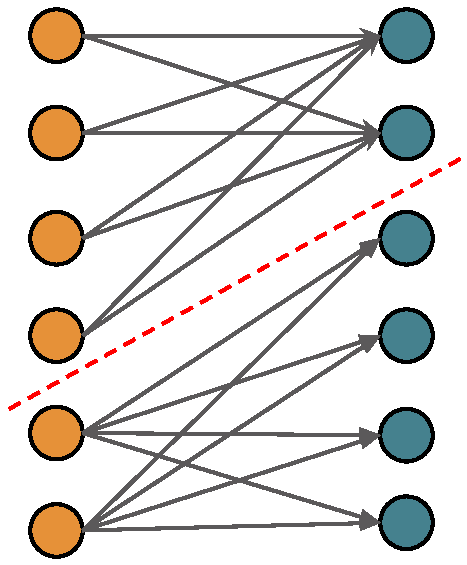
\includegraphics[width=0.55\textwidth]{exchange_part_supreq.pdf}
    \caption[]{
      \label{fig:basic_part}
      A separable bipartite graph with the partition shown as a red 
      dashed line.}
  \end{center}
\end{figure}

The Exchange Graph of the NFCTP, however, has additional structure in the form
of portfolios and thus has a stricter notion of separability. Specifically, the
partition must also separate the set of supplier portfolios, $S$, and requester
portfolios, $R$, as in Equations \ref{eqn:sup_part} and \ref{eqn:req_part},
respectively.

\begin{equation}\label{eqn:sup_part}
  S = S_{1} \cup S_{2}
\end{equation}

\begin{equation}\label{eqn:req_part}
  R = R_{1} \cup R_{2}
\end{equation}

Figure \ref{fig:port_part} depicts a separable Exchange Graph, for example,
while Figure \ref{fig:port_no_part} shows an Exchange Graph that is not
separable, even though the underlying bipartite graph is, due to the lack of a
fully separable portfolio partition.

\begin{figure}
  \begin{center}
    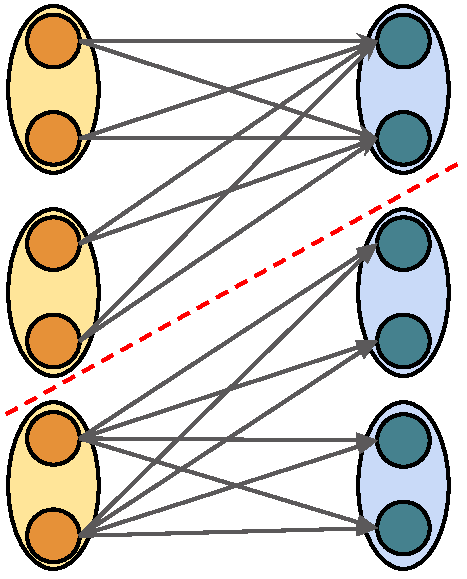
\includegraphics[width=0.55\textwidth]{exchange_part_port.pdf}
    \caption[]{
      \label{fig:port_part}
      A separable Exchange Graph with nodes grouped by portfolio and the
      separating partition shown as a red dashed line.}
  \end{center}
\end{figure}

\begin{figure}
  \begin{center}
    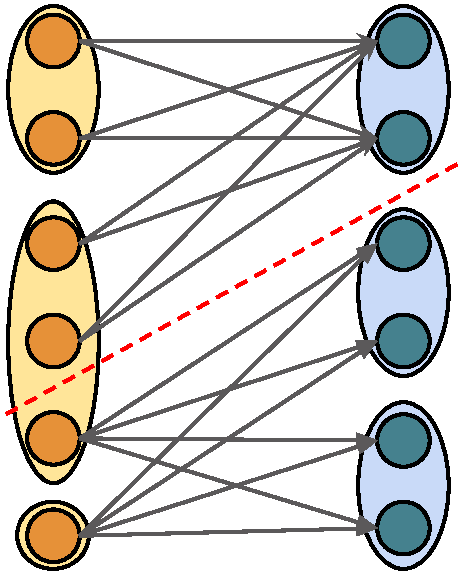
\includegraphics[width=0.55\textwidth]{exchange_no_part_port.pdf}
    \caption[]{
      \label{fig:port_no_part}
      An Exchange Graph with nodes grouped by portfolio that is \textit{not}
      separable because a portfolio crosses the node partition.}
  \end{center}
\end{figure}

The Exchange Graph resulting from the information gathering phase of the DRE
specifically from a NFC application will be minimally separable into front-end
and back-end exchanges if two conditions are met:

\begin{enumerate}
  \item Reactors output commodities can \textit{not} be sent to both other
    reactors and supporting facilities.

  \item Supporting facility output commodities can \textit{not} be sent to both
    other supporting facilities and reactors.
\end{enumerate}

In the first case, separability is broken by a supplier providing bids across a
separating partition. An minimal example is shown in Figure
\ref{fig:no_part_front}. This case can arise if reactors can somehow directly
refuel other reactors. In the NFC domain, such an arrangement only occurs in a
self-recycling system implemented in such a way that a reactor resupplies
itself, which is an abstraction of reality. It is reasonable for a
self-recycling reactor to be implemented in such a way that it does not
participate in the DRE for self-refueling purposes. Accordingly, this condition
is expected to be met in most usage of the DRE.

\begin{figure}
  \begin{center}
    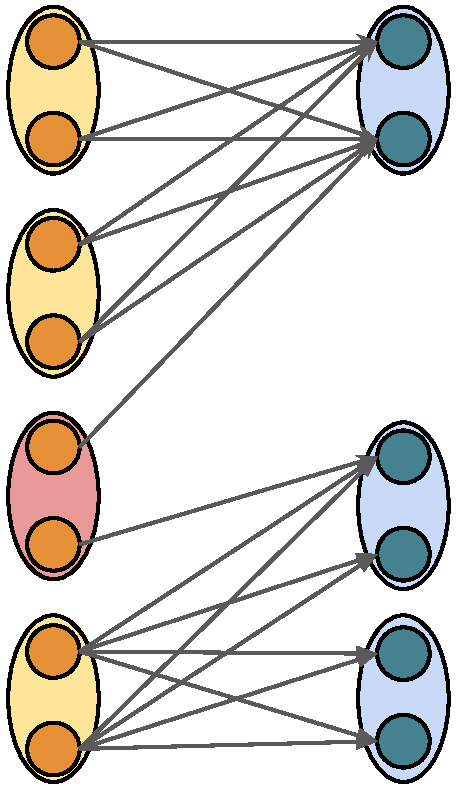
\includegraphics[width=0.55\textwidth]{exchange_no_part_front.pdf}
    \caption[]{
      \label{fig:no_part_front}
      An Exchange Graph separability broken by a supplier. This occurs in NFC
      modeling if assumption $1$ is broken.}
  \end{center}
\end{figure}

In the second case, separability is broken by a requester requesting commodities
across a separating partition. Again, a minimal example is shown in Figure
\ref{fig:no_part_back}. This case can arise in practice when modeling an NFC
system if both a reactor and a repository compete for some commodity. While this
is a valid modeling case under certain assumptions and simplifications, it is
not very realistic. In general fuel that can be used by a reactor has been
processed differently than material to be sent to a repository. Accordingly,
while some analyzed fuel cycles will not meet this requirement, it is assumed
that the vast majority will. If an instance of a DRE does not meet this
requirement, it will not be able to be subdivided into smaller instances.

\begin{figure}
  \begin{center}
    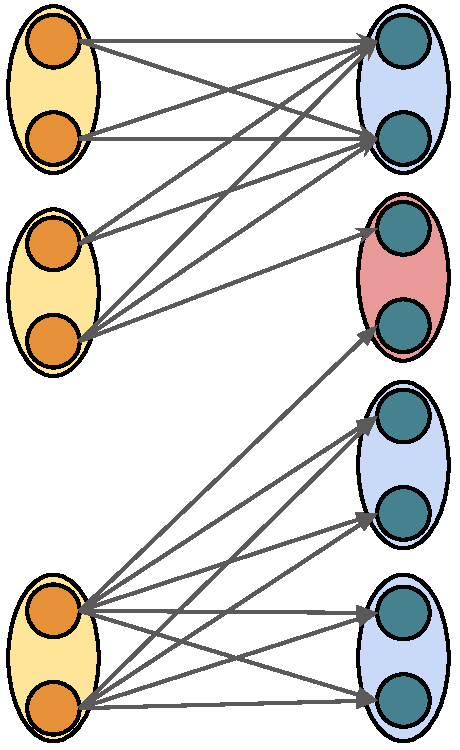
\includegraphics[width=0.55\textwidth]{exchange_no_part_back.pdf}
    \caption[]{
      \label{fig:no_part_back}
      An Exchange Graph separability broken by a requester. This occurs in NFC
      modeling if assumption $2$ is broken.}
  \end{center}
\end{figure}

Because the majority of fuel cycles analyzed will meet both conditions, the
majority of DRE instances will be able to be separated into two distinct
instances which can solved independently of one another. One instance will be
associated with the front end of the fuel cycle where reactors are requesting
fuel. The other instance will be associated with the back end of the fuel cycle,
where reactors are supplying used fuel.

\subsection{Exchange Parameters}\label{method:setup:params}

The generation of exchanges is naturally a parameterized process. For instance,
a fundamental parameter is the number of reactors in an exchange. Exchange
generation parameters can be divided into two classifications, fundamental
parameters and instance parameters. All exchange species share fundmental
parameters, but some species have species-specific instance parameters.

\subsubsection{Fundamental Parameters}

The fundamental parameters are related to the common features of all species
described in \S \ref{method:setup:features}. Each parameter is a switch that
sets the level of fidelity of a given exchange. As such, they are each denoted
as $f_x$, where the $x$ subscript describes the parameter.

The most critical parameter is related to the fidelity of the fuel cycle being
modeled, $f_{fc}$. A value of zero indicates modeling the OT fuel cycle, one is
used for the MOX fuel cycle, and two the ThOX fuel cycle. As fuel cycle fidelity
increases, the number of commodities increases, and thus the number of possible
connections between suppliers and consumers that exist increases as some
entities trade in multiple commodities.

The second parameter is reactor fidelity, $f_{rxtr}$. Reactors can either make
requests or provide supply based either on their entire batch or for each
assembly in a batch. A value of zero indicates reactors trading full batches; a
value of one indicates reactors trading individual assemblies. Trading
individual assemblies is of higher fidelity because the number of trades
increases by nearly an order of magnitude.

Finally, the fidelity with with objective value coefficients are generated can
be varied. This parameter is denoted $f_{loc}$ because it is related to the
degree to which location is taken into account in Equation
\ref{eqn:loc_proxy}. The mapping between $f_{loc}$ and parameters in Equation
\ref{eqn:loc_proxy} is shown in Table \ref{tbl:floc}. As $f_{loc}$ increases,
the size of the distribution of possible objective coefficent values increases.

\begin{table}[h]
\centering
\caption{$f_{loc}$ Effects on Objective Coefficient Values}
\label{tbl:floc}
\begin{tabular}{|c|c|c|c|}
\hline
$f_{loc}$ & $\delta_{reg}$ & $\delta_{loc}$ \\ \hline
0  & 0          & 0 \\ \hline
1   & 1          & 0 \\ \hline
2   & 1          & 0 \\ \hline
\end{tabular}
\end{table}

\subsubsection{Instance Parameters}

\subsection{Front-End Exchanges}\label{method:setup:front}

\subsection{Back-End Exchanges}\label{method:setup:back}

\section{Experimental Tools}\label{method:tools}

\subsection{Structure}\label{method:tools:struc}

\subsection{Persistence Mechanisms}\label{method:tools:hdf5}

what gets recorded

\subsection{High Throughput Computing}\label{method:tools:htc}

Things \cite{bui_work_2011}.
